\documentclass[main.tex]{subfiles}
\begin{document}

% Big schéma
% \imgt{4/6}
\begin{figure}[H]
  \centering
  \begin{tikzpicture}
    \draw (0,0)node[below left]{$x_c(t)$}to[short,o-] ++(1,0)to[spst] ++(2,0) coordinate (E) to[C] ++(0,-2) node[ground]{};
    \draw[dashed] (1,1) rectangle (4,-2) (2.5,1){node[above]{Echantilloneur bloqueur}} ;
    \sbBlocL{can}{CAN}{E}
    \sbBlocL{F}{
      \begin{tabular}{c}
Filtre \\linéaire
      \end{tabular}
    }{can}
    \sbBlocL{cna}{CNA}{F}
    \draw (cna) -- ++(1,0) to[lowpass,-o] ++(2,0) node[below right]{$y_c(t)$};
  \end{tikzpicture}
  \caption{Traitement numérique d'un signal analogique}
\end{figure}
\section{Convertisseur numérique analogique}
\subsection{Principes}
% CNA
\begin{figure}[H]
  \centering
  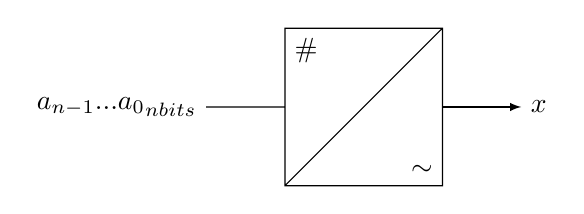
\begin{tikzpicture}
    \draw (0,0) node[left]{$\underbracket{a_{n-1}...a_0}_{\text{n bits}}$} -- (1,0) (1,1)node[below right]{$\#$} rectangle (3,-1)node[above left]{$\sim$} (1,-1) -- (3,1);
    \draw[-latex] (3,0) -- ++(1,0) node[right]{$x$};
  \end{tikzpicture}
  \[
    x =V_{ref} \sum_{k=0}^{n-1}a_k2^k
  \]
  \caption{principe du CNA}
\end{figure}
\subsection{Caractéristiques de transfert}
\begin{figure}[H]
  \centering
  \begin{tikzpicture}
    \begin{axis}
      [axis lines= middle,
      xmin=0,xmax=6,
      ymin=0,ymax=5,
      xtick={0,1,2,3,4},
      xticklabels={00,01,10,11},
      x tick label as interval,
      ytick={1,2,3},
      domain=0:4,
      yticklabels={$V_{ref}$,$2V_{ref}$,$3V_{ref}$},
      ]
      \addplot[dashed,black]{x};
      \addplot[black,thick] plot coordinates
       {(0,0)(1,0)(1,1)(2,1)(2,2)(3,2)(3,3)(4,3)};
    \end{axis}
  \end{tikzpicture}
  \caption{résolution du convertisseur}
\end{figure}

Résolution du convertisseur = impact du bit $a_0$ (LSB) = quantum de conversion :
\[ q = \frac{E}{2^n -1} \text{ avec } E = V_{ref} \sum_{k=0}^{n-1} 2^k = V_{ref} (2^n -1) \]

\subsection{Défauts}

\begin{figure}[H]\centering
  \begin{subfigure}{0.3\linewidth}
    \centering
    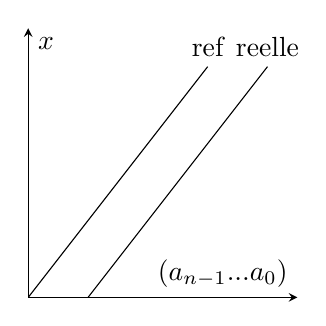
\begin{tikzpicture}
      \begin{axis}
        [axis lines= middle,width=5cm,height=5cm,
        ticks=none,
        xlabel=$(a_{n-1}...a_0)$,
        ylabel=$x$,
        xmin=0,xmax=4.5,ymin=0,ymax=3.5]

      \addplot[black]plot coordinates{(0,0) (3,3)};
      \addplot[black]plot coordinates{(1,0) (4,3)};
      \draw (axis cs:3,3) node[above]{ref}
      (axis cs:4,3) node[above]{reelle};
      \end{axis}
    \end{tikzpicture}
    \subcaption{Erreur de décalage}
  \end{subfigure}%
  \begin{subfigure}{0.3\linewidth}
    \centering
    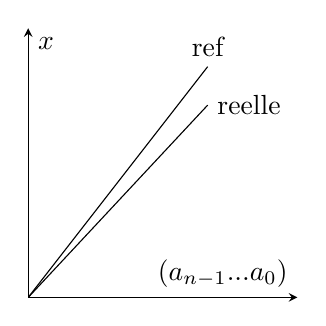
\begin{tikzpicture}
      \begin{axis}
        [axis lines= middle,width=5cm,height=5cm,
        ticks=none,
        xlabel=$(a_{n-1}...a_0)$,
        ylabel=$x$,
        xmin=0,xmax=4.5,ymin=0,ymax=3.5]

      \addplot[black]plot coordinates{(0,0) (3,3)};
      \addplot[black]plot coordinates{(0,0) (3,2.5)};
      \draw (axis cs:3,3) node[above]{ref}
      (axis cs:3,2.5) node[right]{reelle};
      \end{axis}
    \end{tikzpicture}
    \subcaption{Erreur de gain}
  \end{subfigure} \\

  \begin{subfigure}{0.3\linewidth}
    \centering
    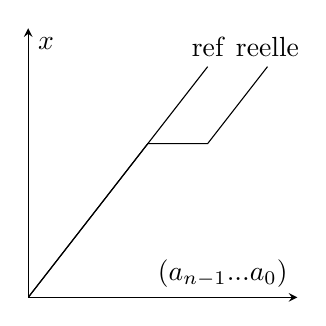
\begin{tikzpicture}
      \begin{axis}
        [axis lines= middle,width=5cm,height=5cm,
        ticks=none,
        xlabel=$(a_{n-1}...a_0)$,
        ylabel=$x$,
        xmin=0,xmax=4.5,ymin=0,ymax=3.5]

      \addplot[black]plot coordinates{(0,0) (3,3)};
      \addplot[black]plot coordinates{(0,0) (2,2)(3,2) (4,3)};
      \draw (axis cs:3,3) node[above]{ref}
      (axis cs:4,3) node[above]{reelle};
      \end{axis}
    \end{tikzpicture}
    \subcaption{Erreur de linéarité}
  \end{subfigure}%
\begin{subfigure}{0.3\linewidth}
    \centering
    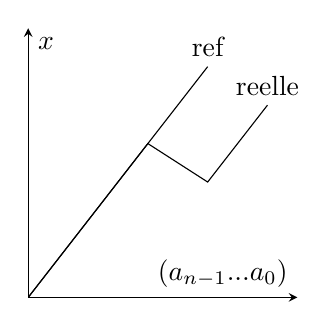
\begin{tikzpicture}
      \begin{axis}
        [axis lines= middle, width=5cm,height=5cm,
        ticks=none,
        xlabel=$(a_{n-1}...a_0)$,
        ylabel=$x$,
        xmin=0,xmax=4.5,ymin=0,ymax=3.5]

      \addplot[black]plot coordinates{(0,0) (3,3)};
      \addplot[black]plot coordinates{(0,0) (2,2) (3,1.5) (4,2.5)};
      \draw (axis cs:3,3) node[above]{ref}
      (axis cs:4,2.5) node[above]{reelle};
      \end{axis}
    \end{tikzpicture}
    \subcaption{Erreur de monotonicité}
  \end{subfigure}

\caption{Différentes erreurs possibles}
\end{figure}
Pour l'erreur  de monotonicité, plusieurs séquence de bits conduisent à une même valeur analogique.

Ce sont des défauts n'apparaissant pas systématiquement mais qui peuvent apparaître en transitoire ou à mesure que le convertisseur se dégrade en fonctionnement.

On a les mêmes problèmes possibles sur les CAN, induits par des problèmes de fiabilité dans l'utilisation des convertisseurs, voire de variabilité sur les technologies CMOS les plus avancées (sensibles à des défauts à l'échelle d'un atome).

\subsection{Réalisation}

\paragraph{Structures directes à courants pondérés}

\begin{itemize}

\item Principe
%\img{0.5}{4/13}
\begin{figure}[H]
  \begin{center}
    \begin{subfigure}{0.45\linewidth}
      \centering
    \begin{tikzpicture}
      \foreach \y/\l in {-3/0,-2/1,0/k,1/n-2,2/n-1}
      {\draw (0,\y)to[spst,l=$a_{\l}$] ++(1,0) to[I,i={$2^{\l}I_0$}]++(3,0);}
      \draw (0,-3) -- (0,-2) (4,-3)--(4,-2)
            (0,0) --(0,2) (4,0) --(4,2);
      \draw[dashed] (0,-2) --(0,0) (4,-2)--(4,0);
      \draw (0,0) -- ++(-0.5,0)
      (4,0) to[R,l_=$R$,v^<=$x$] ++(2,0) node[ground]{};
    \end{tikzpicture}
    \subcaption{Schéma théorique}
  \end{subfigure}%
  \begin{subfigure}{0.55\linewidth}
    \begin{tikzpicture}
      \foreach \y/\l in {-3/0,-2/1,0/k,1/n-2,2/n-1}
      {\draw (0,\y)to[spst,l=$a_{\l}$] ++(1,0) to[R,l={$2^{\l}I_0$}]++(3,0);}
      \draw (0,-3) -- (0,-2) (4,-3)--(4,-2)
            (0,0) --(0,2) (4,0) --(4,2);
      \draw[dashed] (0,-2) --(0,0) (4,-2)--(4,0);
      \draw (0,0) node[above left]{$V_{DD}$} to[o-] ++(-1,0)
      (4,0) -- ++(0.5,0) to[R,l_=$R$,v^<=$x$] ++(3,0) node[ground,rotate=90]{};
      \draw (6,-2) node[op amp](A){}
      (A.-) -| (4.5,0)
      (A.+) -- ++(-0.4,0) -- ++(0,-0.5) node[ground]{}
      (A.out) -| (7.5,0);
    \end{tikzpicture}
    \subcaption{Mise en pratique}
  \end{subfigure}
\end{center}
\caption{CNA}
\end{figure}

\begin{enumerate}[label=(\alph*)]
\item

Conduit à une conversion très rapide. Cependant dans la réalité on ne relie pas une source de courant à un interrupteur. Sinon boum.

  \[
    V_s = -RI = - R.(2^{n-1}I_0a_{n-1}+2^{n-2}I_0a_{n-2}+ ... + 2I_0a_1+I_0a_0) = -RI_0 \sum_{i=0}^{n-1}2^ia_i
\]
\item
En pratique on utilise des résistances:

  \[
    I = \frac{V_{ref}}{R_0}a_{n-1}+\frac{V_{ref}}{2R_0}a_{n-2} + ...+ \frac{V_{ref}}{2^{n-1}R_0}a_{0} = \frac{V_{ref}}{2^{n-1}R_0}\left(2^{n-1}a_{n-1}+...2a_1+a_0\right)\]

\[
  V_{s} = \frac{V_{ref}}{2^{n-1}}\frac{R}{R_0}A
\]

\end{enumerate}

Simple mais plus le nombre de bits augmente, plus on a besoin de résistances de valeurs différentes et grandes.

Problèmes de variabilité et d'intégration. OK jusqu'à 4 bits peut-être, pas vers l'infini et au-dela.

\begin{rem}
  Lors du passage de $A=2^{n}-1$ à $2^n$ tous les interrupteurs doivent commuter simultanément s'il y a disparité , apparition de glitch.
\end{rem}


\item Réseau R-2R

  % \img{0.5}{4/15}
  \begin{figure}[H]
    \centering
    \begin{tikzpicture}
      \draw (-1,0) node[left]{$V_{DD}$} to[short,*-] (0,0)
      to[R,l=$R$]++(2,0)
      to[R,l=$R$]++(2,0)
      to[R,l=$R$]++(2,0)
      to[R,l=$2R$]++(2,0) node[ground,rotate=90]{};
      \node[op amp] (A) at (8,-4.5){};
      \foreach \x/\l in {0/0,2/1,4/2,6/3}
      {\draw (\x,0) to[R,l=$2R$]++(0,-2)++(0,-0.5) node[spdt,rotate=-90,](s-\x){} node[right=0.8em]{$a_\l$};
        \draw (s-\x.out 1) |- (A.-) (s-\x.out 2) node[ground]{};
      }
      \draw (A.+)-- ++(0,-0.5) node[ground]{} (A.-) -- ++(0,1) to[R,l=$R$]++(2.5,0) |- (A.out) to[short,-o]++(1,0);
      \end{tikzpicture}
  \caption{Structure R-2R}
\end{figure}
Même résultat mais avec 2 valeurs de résistances à contrôler qui peuvent être faibles.
\end{itemize}

\paragraph{Structure à conversion indirecte}.\\
Pour de la conversion indirecte on passe par une l'utilisation d'une PWM qui peux être analogiue ou numérique:
\begin{figure}[H]
  \centering
  \begin{tikzpicture}
    \draw (0,0) node[op amp](AO){}
    (AO.out) node[right](AOout){};
    \begin{axis}[
      at={(AO.-)}, anchor=south east,
      height=3cm,width=5cm,
      axis lines =middle,
      ylabel=$V_+$,ylabel style={anchor=south},
      xlabel=$t$,ticks=none,
      xmin=0, xmax=4.5,ymin=-2,ymax=2]
      \addplot[black] plot coordinates {(0,-2) (2,2)(2,-2)(4,2)(4,-2)};
    \end{axis}
\begin{axis}[
      at={(AO.+)}, anchor=north east,
      height=3cm,width=5cm,
      axis lines =middle,
      ylabel=$V_-$,ylabel style={anchor=south},
      xlabel=$t$,,ticks=none,
      xmin=0, xmax=4.5,ymin=-2,ymax=2]
      \addplot[black] plot coordinates {(0,1.5) (4,1.5)};
    \end{axis}
    \begin{axis}[
      at={(AOout)++(1,0)}, anchor=west,
      height=3cm,width=5cm,
      axis lines =middle,
      ylabel=$V_s$, ylabel style={anchor=south},
      xlabel=$t$,xtick=\empty,ytick={-2,2},yticklabels={+E,-E},
      xmin=0, xmax=4.5,ymin=-2,ymax=2]
      \addplot[black, dashed] plot coordinates {(0,1.5) (4,1.5)};
      \addplot[black, dashed] plot coordinates {(0,-2) (2,2)(2,-2)(4,2)(4,-2)};
      \addplot[black] plot coordinates {(0,2) (1.8,2) (1.8,-2) (2,-2) (2,2) (3.8,2) (3.8,-2)};
    \end{axis}
  \end{tikzpicture}
  \caption{PWM analogique}
\end{figure}

On peux également également le faire de manière entièrement numérique(avec un compteur modulo N) mais retard systématique entre l'entrée et la sortie de $2^n T_e$.
Le concept est similaire a l'amplification de classe D.


\section{Convertisseur analogique numérique}

\subsection{Principes et défauts}

Exemple de quantification :
%\img{0.3}{5/1}

À une certaine plage de variation de $x_E$ on associe une valeur quantifiée $\Delta_k$ parmi $n$ valeurs possibles.

Si $x_E \in ]\Delta_k - \frac{p_k}{2}, \Delta_k + \frac{p_k}{2}]$, alors $\Delta = \Delta_k$ où $p_k=\Delta_{k+1} - \Delta_k$ pas de quantification.

\begin{rem}
Par la suite sur la 1e partie de 433, on ne considérera que des quantifications à pas constant : \[\Delta_{k+1}-\Delta_k=q\]

Dans la 2e partie de 433, on étudiera des stratégies à pas non uniformes, souvent utilisées dans les télécoms (pas faible pour les petites valeurs de signal, plus important pour les grandes valeurs).
\end{rem}

$2v_{max}=E$ plage de conversion

Puis codage des $n$ valeurs quantifiées sur $N$ bits (avec $2^N-1\geq n$)

\begin{exemple}

$\Delta_0 \to 0\dots00$

$\Delta_1 \to 0\dots01$

$\Delta_2 \to 0\dots10$
\end{exemple}

On a \[q=\frac{E}{2^N-1}\]

Défauts possibles ? Les mêmes que pour les CNA : erreurs de gain, de linéarité...



\subsection{Bruit de quantification}

$b_q=x_E-\Delta_k$ varie de $-q/2$ à $q/2$ dans le cas de l'exemple de quantification précédent.

Cet écart systématique est traité dans les systèmes électroniques comme un bruit de quantification pour évaluer son impact sur les grandeurs de sortie.

\paragraph{Calcul de la puissance de bruit} Généralement fait dans le cas où $x_E(t)$ évolue linéairement par rapport au temps,  de $-V_{max}$ à $V_{max}$

%\img{0.5}{5/2}
%\img{0.5}{5/3}

\[<b_q>=0 \text{ et } <b_q^2>=\frac{1}{T_q} \int_0^{T_q} b_q^2(t) dt = \frac{q^2}{12}\]

\paragraph{Rapport signal à bruit}
\begin{align*}
RSB_q & = 10 \log \frac{<x_c^2>}{<b_q^2>} \\
RSB_q & = 10 \log( \frac{12(2^N-1)^2}{E^2}<x_c^2>) \\
RSB_q & = N 20 \log 2 + 10 \log 12 + 10 \log \frac{<x_c^2>}{E^2} \quad \text{en supposant } 2^N >>1\\
& \approx 6N + 10,77 + 10 \log \frac{<x_c^2>}{E^2}
\end{align*}

On s'arrête là c'est-à-dire qu'on peut calculer un nombre minimal de bits nécessaires pour que $RSB_q$ dépasse une valeur limite donnée, si $<x_c^2>$ est connu

Si $<x_c^2>$ n'est pas connu, on utilise souvent une expression approchée de $RSB_q$, celle obtenue quand $x_c(t) = \frac{E}{2} \cos(2\pi f t)$

$<x_c^2> = E^2/8$ et $RSB_q = 6N+1,8$

\begin{rem}
Parfois, on rajoute à cette expression un facteur de crête $F_c$ (en dB) et la formule devient \[RSB_q=6N+1,8-F_c\]
où $F_c$ représente l'influence des dépassements possibles de $x_c$ par rapport à la plage de conversion mais aussi de la forme de $x_c$...

$F_c$ : marge d'erreur sur la validité de la formule en $6N+1,8$ qu'on peut évaluer de façon empirique
\end{rem}


\section{Réalisation des CAN}

\subsection{Structures directes : convertisseurs flash ou semi-flash}

Flash : générer l'ensemble des valeurs $\Delta_k$ possibles et les comparer en même temps à $x_E$ : conversion immédiate

\begin{exemple}[Flash pour n=7]
%\img{0.3}{5/4}
\end{exemple}

Rapide mais nécessite $2^N-1$ comparateurs de tension : $N=12$ au grand maximum en pratique.

Moins de comparateurs avec une structure semi-flash :
%\img{0.3}{5/5}

Au lieu de 255 comparateurs pour une flash 8 bits

\subsection{Convertisseur à approximations successives}
%\img{0.3}{5/6}

Pas aussi rapide que la flash mais peut être intégré en CMOS

Stratégie :
\begin{itemize}
\item on commence avec $a_3=1$, $a_2=a_1=a_0=0$
\item si $x_E \geq x_a$ alors on maintient $a_3 = 1$ sinon $a_3=0$.
\item on itère avec $a_2 a_1 $ et $a_0$ mis successivement à 1 (on procède par dichotomie)
\end{itemize}

\begin{rem}
on peut remplacer la logique de contrôle par un simple compteur qui s'arrête dès que $x_E \geq x_a$. Cependant le temps de conversion varie alors de $T_h$ à $(2^N-1)T_h$. Le temps de conversion est donc non-contrôlé et peut devenir très grand devant $T_h$.
\end{rem}

\subsection{Convertisseur à rampe (analogique)}

\begin{itemize}
\item Convertisseur à simple rampe :

%\img{0.25}{5/7}
%\img{0.3}{5/8}


On compte tant que $x_E \geq r$, on obtient les bits associés à $x_E$ et on remet l'intégrateur à 0.

On a un nombre de périodes d'horloges $M=\lfloor\frac{T_c}{T_h}\rfloor$ avec $T_c = \frac{RC}{V_{ref}}$

Cette solution est simple, assez rapide, mais très sensible aux dérives sur les valeurs de R et C.

\item Convertisseur à double rampe

%\img{0.3}{5/9}
%\img{0.3}{5/10}

À $t_1$ fixé, l'interrupteur 1 bascule de $x_E$ à $-V_{ref}$.
À $t_2$, c'est la fin de la conversion, l'intégrateur a été ramené à 0 par l'interrupteur 2.


$t_2$ est tel que \[0=r(t_2) = \frac{-x_E}{RC}t_1 + \frac{V_{ref}}{RC}(t_2-t_1)\] d'où $\frac{t_2-t_1}{t_1} = \frac{x_E}{V_{ref}}$ : indépendant de R et C, possibilité de grande précision de conversion.
\end{itemize}


\subsection{Convertisseur $\Delta$ et $\Sigma\Delta$}

\begin{itemize}
\item Idée : comparer $x_E$ à la sortie d'un intégrateur de pente $q= \pm\frac{V_{ref}}{2RC}$

%\img{0.5}{5/11}

Si $x_c \leq r$, on a une pente de $-\frac{V_{ref}}{2RC}$ à la période $T_H$, si $x_c > r$ on a une pente de $+\frac{V_{ref}}{2RC}$

$\rightarrow$ convertisseur différentiel : on code la dérivée de $x_c$

%\img{0.5}{5/12}

Q code le sens de variation de $x_c$, 1 seul bit est nécessaire.

On doit avoir \[|\frac{dx_c}{dt}| \leq \frac{V_{ref}}{2RC}\]

\item Convertisseur $\Sigma\Delta$ :
permet de pallier cette limitation en intégrant $x_c$ avant de passer par le convertisseur $\Delta$ : \[\frac{1}{\tau}x_c \leq \frac{V_{ref}}{2RC}\] $\tau$ est la grandeur caractéristique de l'intégration.


\end{itemize}
\end{document}

%%% Local Variables:
%%% mode: latex
%%% TeX-master: "main"
%%% End:
